\section{CUDA 动态并行}
CUDA 动态并行性是 CUDA 编程模型的扩展,它使内核能够调用其他内核,从而允许在设备上执行的线程启动新的线程网格。 
在 CUDA 的早期版本中,网格只能从主机代码启动。 
涉及递归、不规则循环结构、时空变化或其他不适合平面和单级并行性的结构的算法需要通过主机的多个内核调用来实现,
这增加了主机的负担、数量 主机设备通信的数量以及总执行时间。 
在某些情况下,程序员诉诸循环序列化和其他笨拙的技术来支持这些算法需求,但以软件可维护性为代价。 
对动态并行性的支持允许动态发现新工作的算法来准备和启动新网格,而不会增加主机负担或影响软件可维护性。 
本章介绍了支持动态并行性的 CUDA 扩展功能,包括对 CUDA 编程接口的修改和添加,以及利用这种附加功能的指南和最佳实践。

\subsection{背景}
\begin{figure}[H]
	\centering
	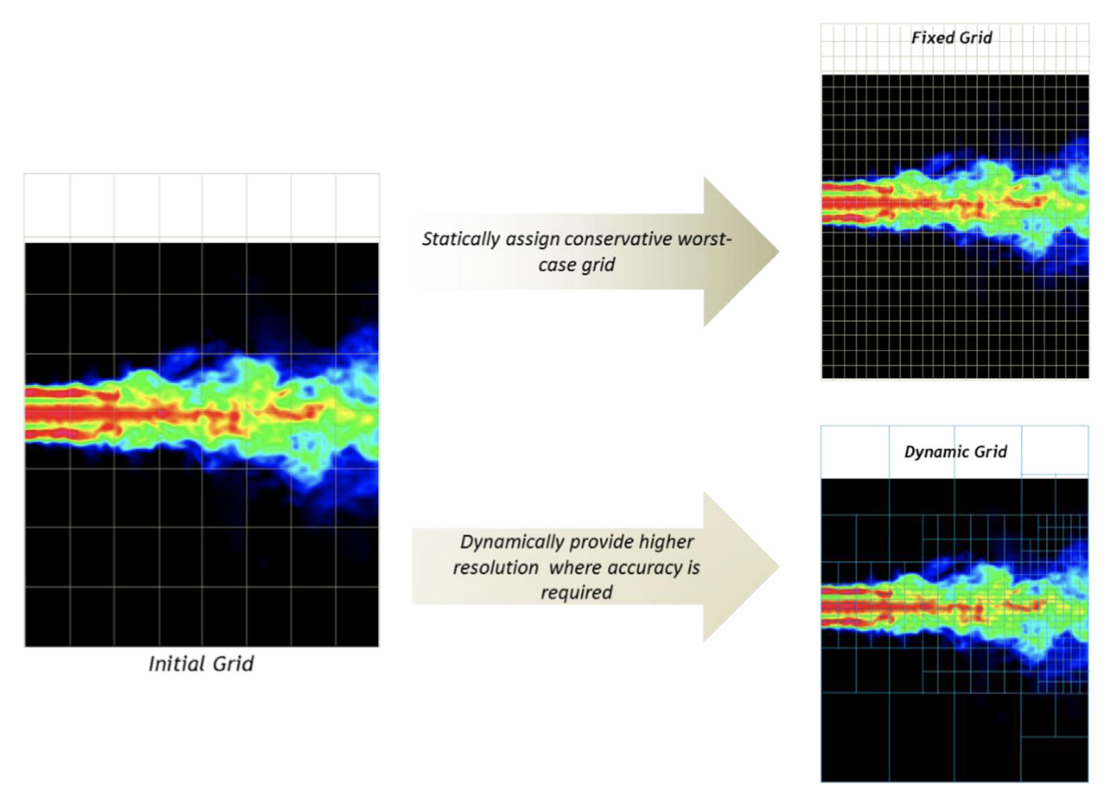
\includegraphics[width=0.9\textwidth]{figs/F21.1.png}
	\caption{\textit{湍流模拟模型的固定网格与动态网格。}}
\end{figure}

许多现实世界的应用程序采用的算法要么具有跨空间的工作变化,要么随着时间的推移动态变化的工作量。 
例如,图 21.1 显示了一个湍流模拟示例,其中所需的建模细节水平随空间和时间的不同而变化。 
随着燃烧流从左向右移动,活动范围和强度增加。 模型右侧建模所需的细节级别远高于模型左侧。 
一方面,使用固定的精细网格会产生过多的工作,而模型的左侧却没有任何增益。 
另一方面,使用固定的粗网格会牺牲模型右侧太多的精度。 
理想情况下,应该对模型中需要更多细节的部分使用精细网格,对不需要更多细节的部分使用粗网格。

到目前为止,我们假设所有内核都是从主机代码调用的。 线程网格完成的工作量是在调用内核函数时预先确定的。 
对于内核代码的单程序、多数据编程风格,让线程块使用不同的网格间距即使不是极其困难,也是乏味的。 
因此,这种限制有利于使用固定且统一(规则)的网格系统。 
为了达到所需的精度,如图 21.1 右上部分所示,这种固定网格方法通常需要适应模型中要求最高的部分,
并维护不必要的额外数据,并在以下部分执行不必要的额外工作: 不需要那么多细节。

更理想的方法如图 21.1 右下部分的动态网格所示。 
当仿真算法检测到模型某些区域中快速变化的仿真量时,它会细化这些区域中的网格以达到所需的精度水平。 
对于没有表现出如此密集活动的区域,不需要进行这种细化。 
因此,该算法可以动态地将更多计算资源引导到从额外工作中受益的模型区域。

\begin{figure}[H]
	\centering
	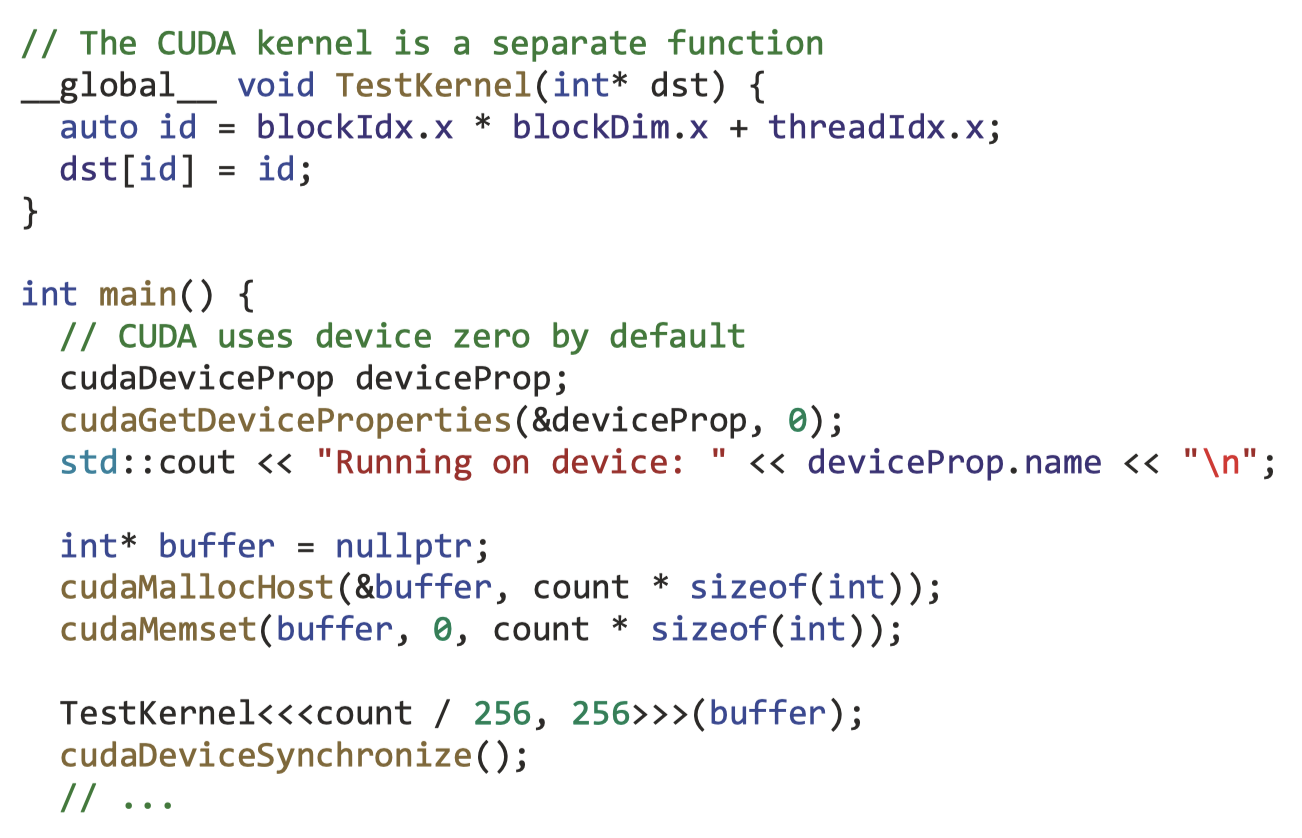
\includegraphics[width=0.9\textwidth]{figs/F21.2.png}
	\caption{\textit{具有动态工作变化的算法的网格启动模式,(A) 不具有动态并行性,(B) 具有动态并行性。}}
\end{figure}

图 21.2 显示了没有动态并行性的系统和另一个具有动态并行性的系统相对于图 21.1 中的仿真模型的行为的概念比较。 
如果没有动态并行性,主机线程必须启动所有网格。 
如果发现新的工作,例如在网格执行期间细化模型中的某个区域,则网格需要终止,向主机报告,并让主机启动新的网格。 
这如图 21.2A 所示,其中主机启动一个网格,在其终止后从该网格接收信息,并为已完成的网格发现的任何新工作启动后续网格。 
该图描绘了相继启动的后续网格; 然而,可以应用复杂的优化,
例如在不同的流中启动独立的网格或将它们组合起来以便它们可以并行运行。

图 21.2B 显示,通过动态并行,发现新工作的线程可以继续并启动网格来完成工作。 
在我们的示例中,当线程发现模型中的某个区域需要细化时,它可以启动一个新网格来对细化区域执行计算,
而无需终止网格、向主机报告并让 主机启动新网格。

\subsection{动态并行概述}
\begin{figure}[H]
	\centering
	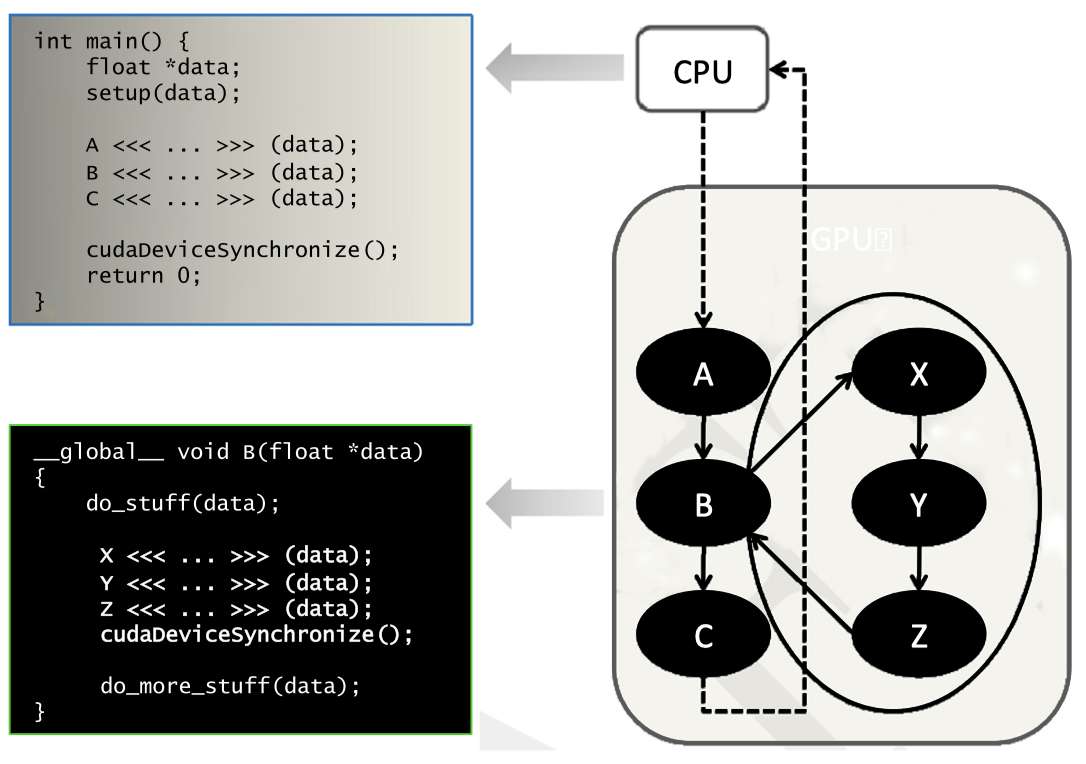
\includegraphics[width=0.9\textwidth]{figs/F21.3.png}
	\caption{\textit{内核 (B) 启动三个内核(X、Y 和 Z)的简单示例。}}
\end{figure}

从程序员的角度来看,动态并行意味着他们可以在一个内核中编写一条调用另一个内核函数的语句。 
在图 21.3 中,主函数(主机代码)启动了三个内核:A、B 和 C。正如我们在整本书中所假设的那样,这些是主机代码中的内核调用。 
图 21.3 中的新内容是内核之一 B 调用三个内核 X、Y 和 Z。这在不支持动态并行性的早期 CUDA 系统中是非法的。 
从内核内部调用内核的语法与从主机代码调用内核的语法相同:

{\color{red} Fig}
kernel\_name<<<D g, D b, N s, S>>([内核参数])

\begin{itemize}
   \item Dg 的类型为 dim3,指定网格的维度和大小。
   \item Db 的类型为 dim3,指定每个线程块的维度和大小。
   \item Ns 的类型为 size\_t,指定为此调用动态分配的每个线程块的共享内存的字节数,这是除了静态分配的共享内存之外的。 
   		Ns 是一个可选参数,默认为 0 。
   \item S 的类型为 cudaStream\_t 并指定与此调用关联的流。 该流必须已分配在进行调用的同一线程块中。 
   		S 是一个可选参数,默认为 0 。 第 20 章“异构计算集群编程”中讨论了流。
\end{itemize}

为了演示如何使用动态并行性,我们提供了不带动态并行性和带动态并行性的内核的简单示例。 
这些示例基于假设的并行算法,该算法不计算有用的结果,但提供了在许多应用程序中重复出现的概念上简单的计算模式。 
它说明了两种方法之间的差异,以及当算法中每个线程完成的工作量可以动态变化时,
如何使用动态并行性来提取更多并行性,同时减少控制流发散。

\begin{figure}[H]
	\centering
	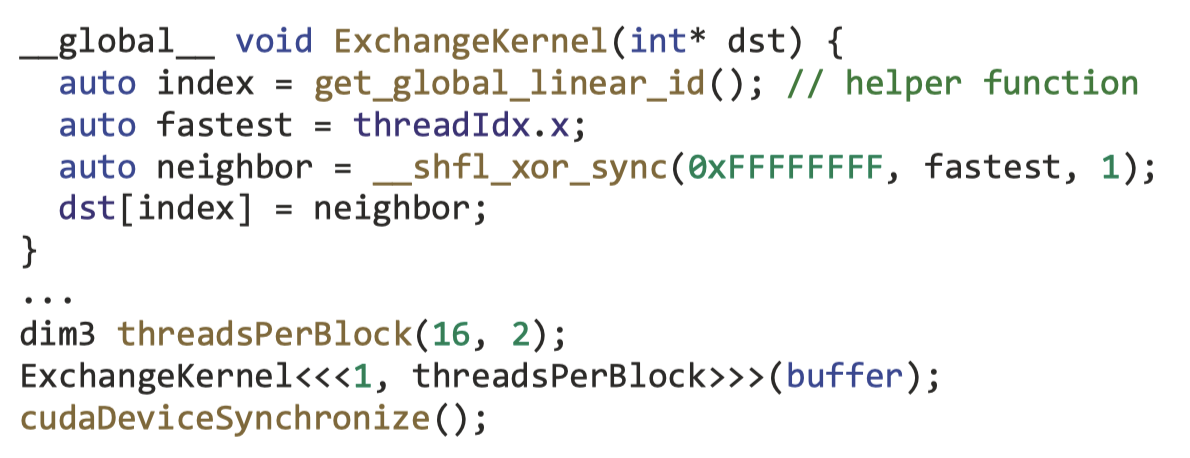
\includegraphics[width=0.9\textwidth]{figs/F21.4.png}
	\caption{\textit{一个用 CUDA 编码的假设并行算法的简单示例,没有动态并行性。}}
\end{figure}

图 21.4 显示了一个没有动态并行编码的简单内核示例。 在此示例中,内核的每个线程执行一些计算(第 05 行),
然后循环遍历其负责的数据元素列表(第 07 行),并对每个数据元素执行另一次计算(第 08 行)。

这种计算模式在许多应用程序中频繁出现。 例如,在图搜索中,每个线程可以访问一个顶点,然后循环遍历相邻顶点的列表。 
读者应该会发现这个内核结构与图 15.14 中以顶点为中心的 BFS 内核类似。 
又例如,在稀疏矩阵计算中,每个线程可以首先识别一行非零元素的起始位置并循环非零值。 
在诸如本章开头的示例之类的模拟中,每个线程可以首先处理粗网格元素,然后在需要细化网格时循环处理更细的网格元素。

以图 21.4 所示的风格编写应用程序有两个主要问题。 
首先,如果循环中的工作(第 $07-09$ 行)可以并行执行并有利可图,那么我们就错过了从应用程序中提取更多并行性的机会。 
其次,如果同一扭曲中的线程之间循环中的迭代次数差异很大,则由此产生的控制分歧会降低程序的性能。

\begin{figure}[H]
	\centering
	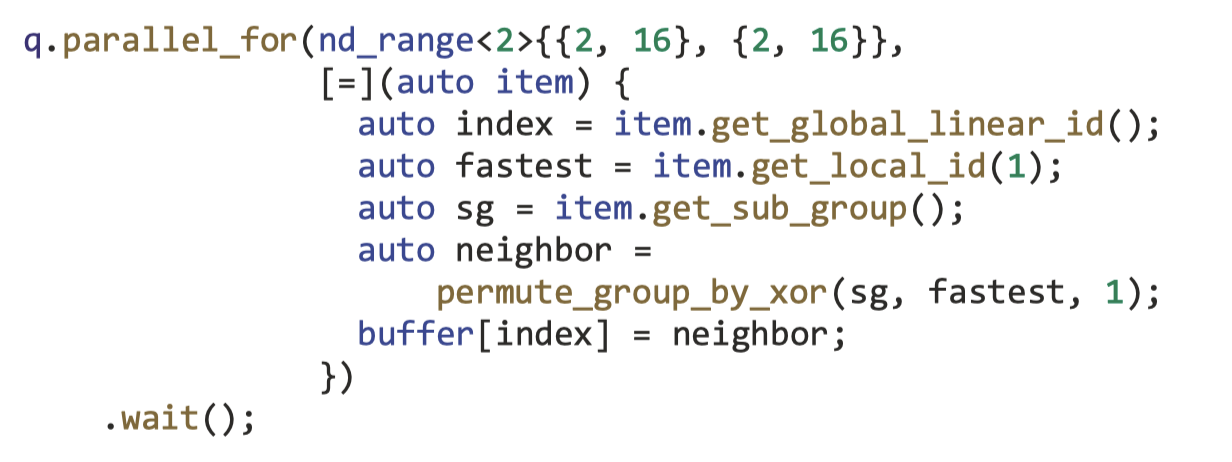
\includegraphics[width=0.9\textwidth]{figs/F21.5.png}
	\caption{\textit{使用 CUDA 动态并行性的修订示例。}}
\end{figure}

图 21.5 显示了使用动态并行性的同一程序的一个版本。 在此版本中,原始内核分为两个:父内核和子内核。 
父内核的启动方式与原始内核相同,由称为父网格的线程网格执行。 父内核不是循环,而是调用子内核来继续工作(第 07-08 行)。 
子内核由称为子网格的线程网格执行,子网格执行最初在循环体内执行的工作(图 21.5 第 18 行)(图 21.4 第 07-09 行)。

以这种方式编写程序可以解决关于原始代码提到的两个问题。 
首先,循环迭代现在由子内核线程并行执行,而不是由原始内核线程串行执行。 因此,我们从程序中提取了更多的并行性。 
其次,每个线程现在执行单个循环迭代,这会带来更好的负载平衡并消除控制发散。 
虽然这两个目标可以通过程序员以不同方式重写内核来实现,例如,通过使用边缘中心广度优先实现,
但对于某些应用程序来说,这种转换可能会很尴尬、复杂且容易出错。 动态并行性提供了一种表达此类计算模式的简单方法。

\subsection{示例:贝塞尔曲线}
我们现在展示一个更有趣、更有用的例子:样条曲线的自适应细分。 此示例说明了根据工作负载启动不同数量的子网格的情况。 
该示例是计算贝塞尔曲线(Bezier Curves),贝塞尔曲线在计算机图形学中经常用于绘制平滑、直观的曲线,
这些曲线由一组控制点定义,这些控制点通常由用户定义。

从数学上讲,贝塞尔曲线由一组控制点 $\mathbf{P}_{0}$ 到 $\mathbf{P}_{n}$ 定义,
其中 $n$ 称为控制点的阶数 ( $n =1$ 表示线性,2 表示二次,3 表示三次,等等)。 
第一个和最后一个控制点始终是曲线的终点; 然而,中间控制点(如果有)通常不在曲线上。

\subsubsection{线性贝塞尔曲线}
给定两个控制点 $\mathbf{P}_{0}$ 和 $\mathbf{P}_{1}$,线性贝塞尔曲线只是连接这两个点的直线。 
曲线上各点的坐标由以下线性插值公式给出:
$$
\mathbf{B}(t)=\mathbf{P}_{0}+t\left(\mathbf{P}_{1}-\mathbf{P}_{0}\right)=(1-t ) \mathbf{P}_{0}+t \mathbf{P}_{1}, \quad t \in[0, \quad 1]
$$

\subsubsection{二次贝塞尔曲线}
二次贝塞尔曲线由三个控制点 $\mathbf{P}_{0}、\mathbf{P}_{1}$ 和 $\mathbf{P}_{2}$ 定义。 
二次曲线上的点定义为从 $\mathbf{P}_{0}$ 到 $\mathbf{P}_{1}$ 
以及从 $\mathbf{P}_{1}$ 的线性贝塞尔曲线上对应点的线性插值到 $\mathbf{P}_{2}$。 曲线上各点坐标的计算用以下公式表示:
$$
\mathbf{B}(t)=(1-t)\left[(1-t) \mathbf{P}_{0}+t \mathbf{P}_{1}\right]+t\left[ (1-t) \mathbf{P}_{0}+t \mathbf{P}_{2}\right], \quad t \in[0, \quad 1],
$$

可以简化为以下公式:
$$
\mathbf{B}(t)=(1-t)^{2} \mathbf{P}_{0}+2(1-t) t \mathbf{P}_{1}+t^{2} \mathbf{P}_{2}, \quad t \in[0, \quad 1] 。
$$

\subsubsection{贝塞尔曲线计算(无动态并行)}
\begin{figure}[H]
	\centering
	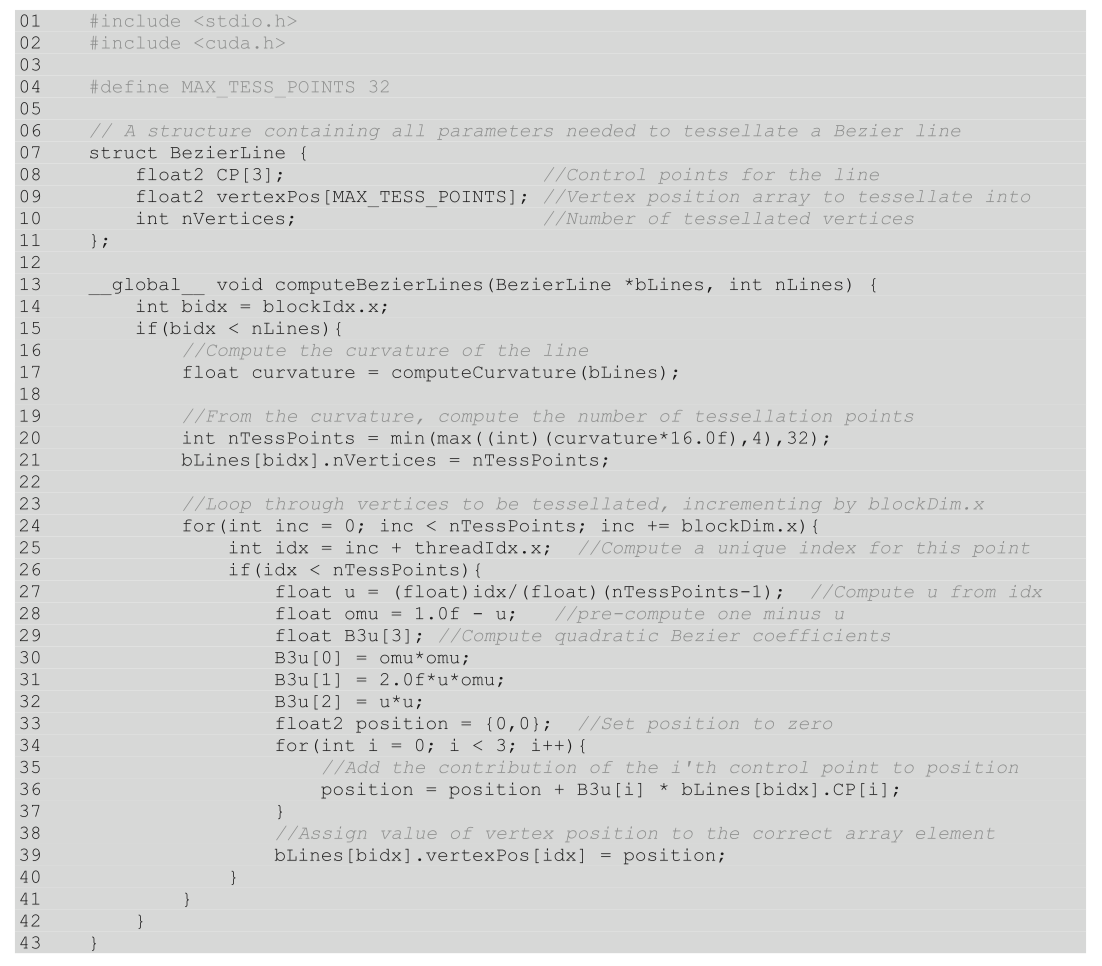
\includegraphics[width=0.9\textwidth]{figs/F21.6.png}
	\caption{\textit{无动态并行性的贝塞尔曲线计算。}}
\end{figure}

图 21.6 显示了计算贝塞尔曲线上点坐标的 CUDA C 程序的一部分。 
从第 13 行开始的computeBeziertines 内核被设计为使用一个块来计算一组三个控制点(二次贝塞尔公式)的曲线点。 
每个线程块首先计算由三个控制点定义的曲线曲率的度量。 直观上,曲率越大,为三个控制点绘制平滑的二次贝塞尔曲线所需的点就越多。 
这定义了每个块要完成的工作量。 这反映在第20行和第21行中,其中当前线程块要计算的总点数与曲率值成正比。

在第 24 行的 for 循环中,所有线程在每次迭代中计算一组连续的贝塞尔曲线点。 循环体中的详细计算基于我们之前提出的公式。 
关键点在于,一个块中的线程所执行的迭代次数可能与另一个块中的线程所执行的迭代次数有很大不同。 
根据调度策略,每个线程块完成的工作量的这种变化可能会导致流式多处理器 (SM) 的利用率降低,从而降低性能。

\subsubsection{贝塞尔曲线计算(具有动态并行性)}
\begin{figure}[H]
	\centering
	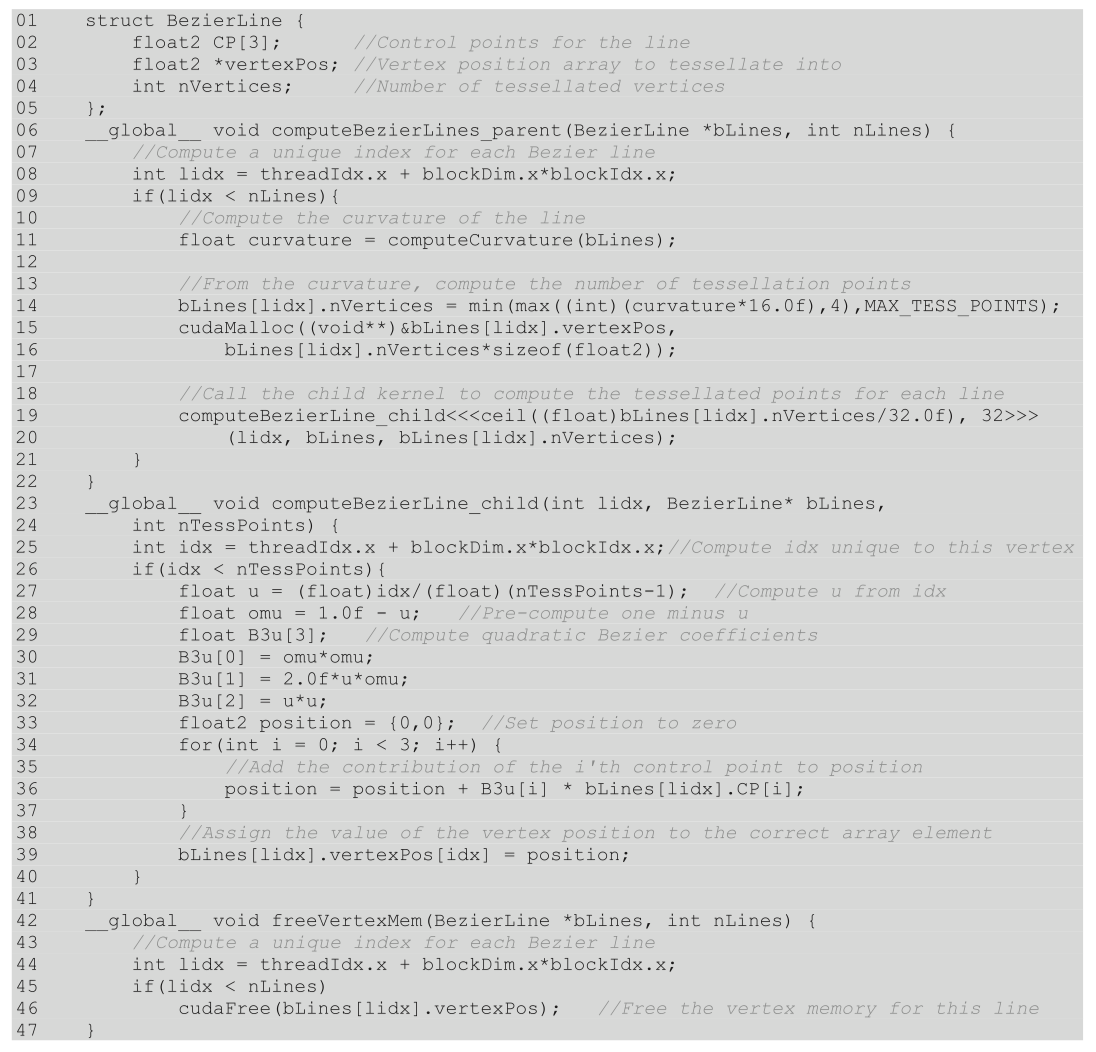
\includegraphics[width=0.9\textwidth]{figs/F21.7.png}
	\caption{\textit{具有动态并行性的贝塞尔计算。}}
\end{figure}

图21.7显示了使用动态并行性的贝塞尔曲线计算代码。 它将图 21.6 中的computeBeziertines 内核分解为两个内核。 
第一部分,computeBezierLines\_parent,发现每个控制点需要完成的工作量。 
第二部分,computeBezierLines\_child,执行计算。

在新的组织中,computeBezierLines\_parent 内核为每组控制点完成的工作量比原始的computeBezierLines 内核要小得多。 
因此,我们在computeBeziertines\_parent 中使用一个线程来完成这项工作,而不是在computeBeziertines 中使用一个块。 
在第 58 行中,我们只需为每组控制点启动一个线程。 
这可以通过将 N\_LINES 除以 BLOCK\_DIM 来形成内核启动配置中的块数来反映。

computeBezierLines\_parent 内核和computeBezierLines 内核之间有两个主要区别。 
首先,用于访问控制点的索引是基于线程(图 21.7 中的第 08 行)而不是基于块(图 21.6 中的第 14 行)形成的。 
这是因为每个控制点的工作是由线程而不是块完成的,正如我们在本章前面提到的。 
其次,用于存储计算出的贝塞尔曲线点的存储器是动态确定和分配的,如图21.7中的第15行所示。 
这允许代码为要放置在 bLines 变量中的每组控制点分配足够的内存。 
请注意,在图 21.6 中,每个 BezierLine 元素都使用最大可能的点数进行声明(第 09 行)。 
另一方面,图 21.7 中的声明只有一个指向动态分配存储的指针。 
在控制点曲率变化很大的情况下,允许内核调用 cudaMa 1 loc () 函数可以显着减少内存使用量。

一旦computeBezierLines\_parent内核的线程确定了其控制点集所需的工作量,
它就会调用computeBezierLines\_child内核并启动子网格来完成工作(图21.7中的第19行)。 
在我们的示例中,父网格中的每个线程都会为其分配的一组控制点创建一个新网格。 这样,每个线程块完成的工作就得到了平衡。 
每个子网格完成的工作量各不相同。

动态并行内核调用与来自主机的内核调用具有相同的异步语义。 
也就是说,一旦子内核被调用,调用它的父线程就可以继续执行后续代码,而无需等待子网格完成。 
如果父线程希望等待其子网格完成,则它必须执行类似于主机线程执行的显式同步。 
如果没有进行显式同步,那么线程可以完成执行,但最后有一个隐式同步。 隐式同步确保所有子网格在父网格终止之前都已终止。 
我们建议读者参阅 CUDA C++ 编程指南,了解有关父子网格同步语义的更多详细信息(NVIDIA Corporation,2021)。

在computeBezierLines\_parent终止后,使用 cudaMalloc 在内核内部分配的内存仍然需要释放。 
因此,实现了一个额外的内核 freevertexMem(第 $42-47$ 行)以供主机调用。 
该内核并行释放分配给 bLines\_d 数据结构中顶点的所有存储(第 61 行)。 
该内核是必要的,因为设备内核在设备上分配的顶点存储必须由设备内核释放。 
我们建议读者参阅 CUDA C++ 编程指南,
了解有关在设备上使用 cudaMalloc 和 cudaFree 的更多详细信息(NVIDIA Corporation,2021)。

\subsection{递归示例:四叉树}
动态并行性还允许程序员实现递归算法。 在本节中,我们将说明如何使用动态并行性来实现四叉树递归(Finkel 和 Bentley,1974)。 
四叉树通过递归地将二维空间细分为四个大小相等的象限来划分二维空间。 每个象限被认为是四叉树的一个节点并且包含多个点。 
如果一个象限中的点数大于固定的最小值,则该象限将被递归地细分为另外四个象限,即四个子节点。

\begin{figure}[H]
	\centering
	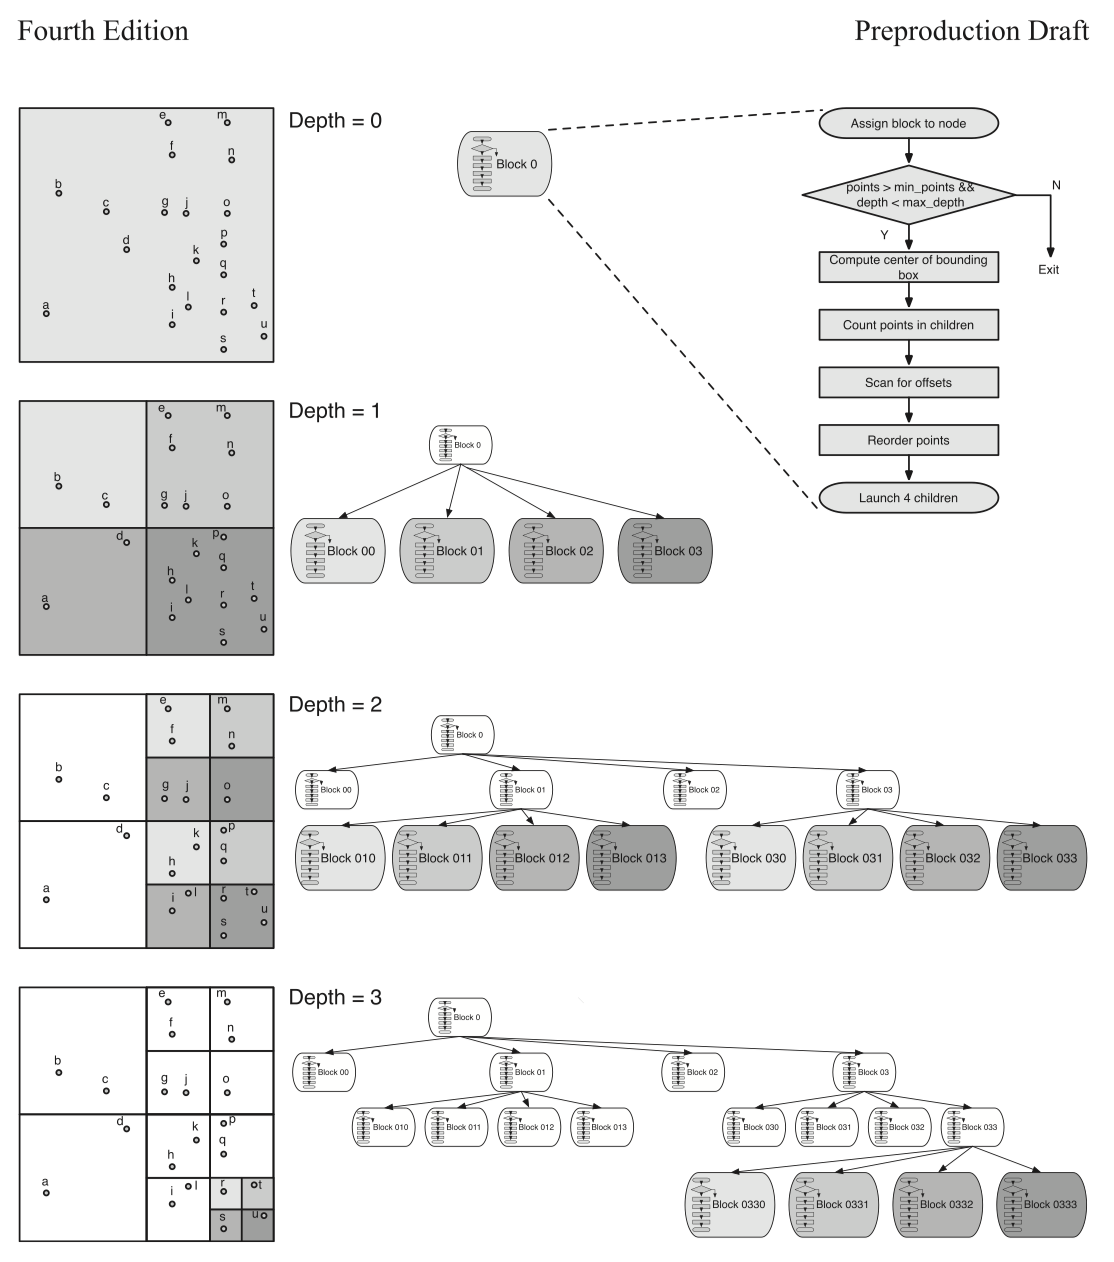
\includegraphics[width=0.9\textwidth]{figs/F21.8.png}
	\caption{\textit{四叉树示例。 每个块被分配到一个象限。 如果象限中的点数多于两个,则该块将启动四个子块。 
	阴影块是每个深度级别中的活动块。}}
\end{figure}

图 21.8 说明了具有动态并行性的四叉树的构造。 在此实现中,一个节点(象限)被分配给一个块。 
最初(depth = 0),一个块(块0)被分配给整个二维空间(四叉树的根节点),其中包含所有点。 
它将空间分为四个象限,并为每个象限发射一个区块(depth = 1)。 
如果这些子块(块 00 到 03)包含的点多于固定的最小值,它们将再次细分其象限。 
在此示例中,我们假设最小值为 2; 因此块 00 和 02 不会启动子块。 01 号区块和 03 号区块推出了一个网格,各有四个区块。

如图21.8右侧的流程图所示,块首先检查其象限内的点数是否大于进一步划分所需的最小值以及是否尚未达到最大深度。 
如果任一条件失败,则象限的工作完成,并且块返回。 否则,该模块将计算围绕其象限的边界框的中心。 中心位于四个新象限的中间。 
计算每个点的点数。 四元素扫描操作用于计算存储点的位置的偏移量。 
然后对这些点重新排序,以便将同一象限中的那些点分组在一起并放入点存储的相应部分中。 
最后,该块启动一个包含四个块的子网格,每个块对应四个新象限。

\begin{figure}[H]
	\centering
	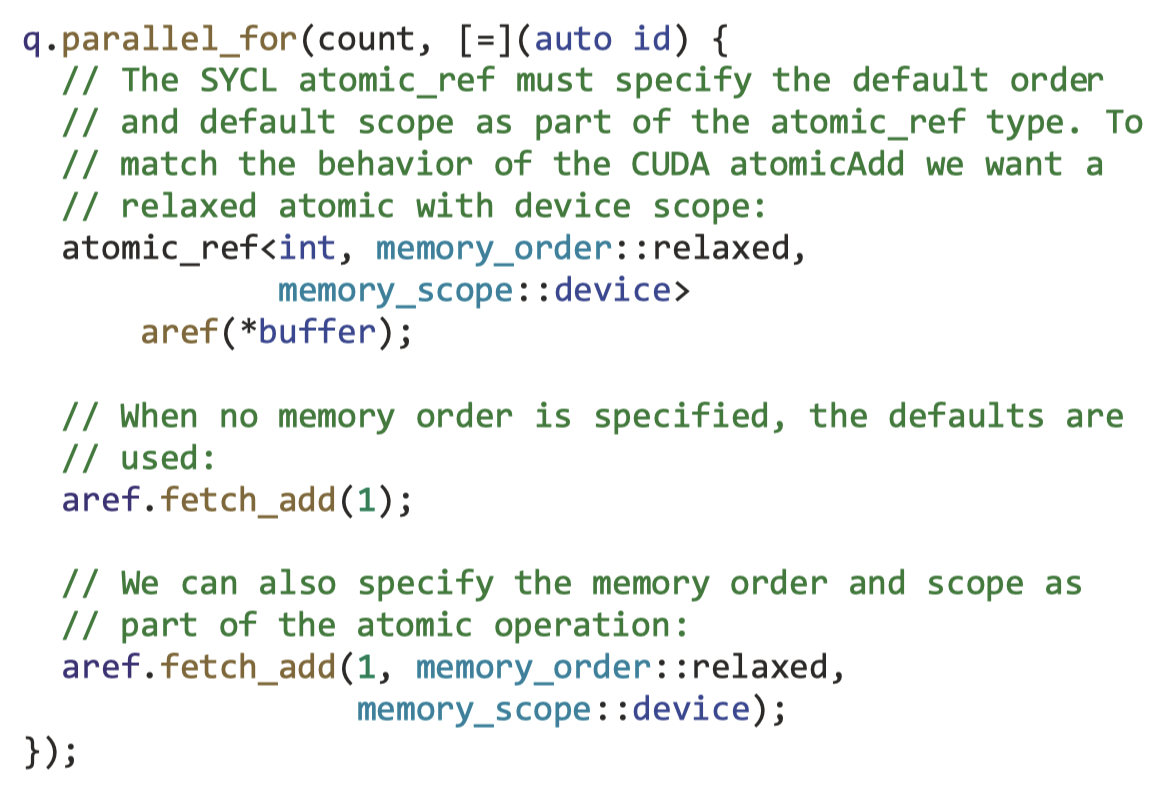
\includegraphics[width=0.9\textwidth]{figs/F21.9.png}
	\caption{\textit{四叉树示例。 在每个深度级别,块将同一象限中的所有点分组在一起。 
	(A) 显示缓冲区 0 中的初始输入列表,(B) 重新排列为对应于四个象限的四个子列表后的列表,
	(C) 显示重新排列以反映第二级象限后的列表,(D) 显示了重新排列以反映第三级象限后的列表,
	(E) 最终列表被复制到缓冲区 0 以返回给调用者。}}
\end{figure}

图 21.9 继续图 21.8 中的小示例,详细说明了如何在每个深度级别对点进行重新排序。 
对于这个例子,我们假设每个象限必须有两个以上的点才能进一步划分。 该算法使用两个缓冲区来存储点并对它们重新排序。 
算法结束时这些点应位于缓冲区 0 中。 因此,如果满足终止条件时点位于缓冲区 1 中,则可能需要在离开之前交换缓冲区内容。

在主机代码的初始内核调用中(深度 = 0),块 0 被分配了驻留在缓冲区 0 中的所有点,如图 21.9A 所示。 
块0进一步将该象限划分为四个子象限,将同一子象限中的所有点分组在一起,并根据象限将点存储到缓冲器1中,如图21.9B所示。 
它的四个子项,块 00 到块 03,被分配给四个新象限中的每一个,如图 21.9B 中标记的范围所示。 
块 00 和 02 不会启动子块,因为它们各自分配的象限中的点数只有 2。
块 01 和 03 重新排序它们的点以将它们分组在同一象限中,并分别启动四个子块,如图 21.9 所示 C。 
块 010、011、012、013、030、031 和 032 不启动子块(它们有两个或更少的点),并且不需要交换点(它们已经在缓冲区 0 中)。 
只有块 033 重新排序其点并启动四个块,如图 21.9D 所示。 
块0330到0333在将它们的点交换到缓冲器0之后将退出,这可以在图21.9E中看到。

\begin{figure}[H]
	\centering
	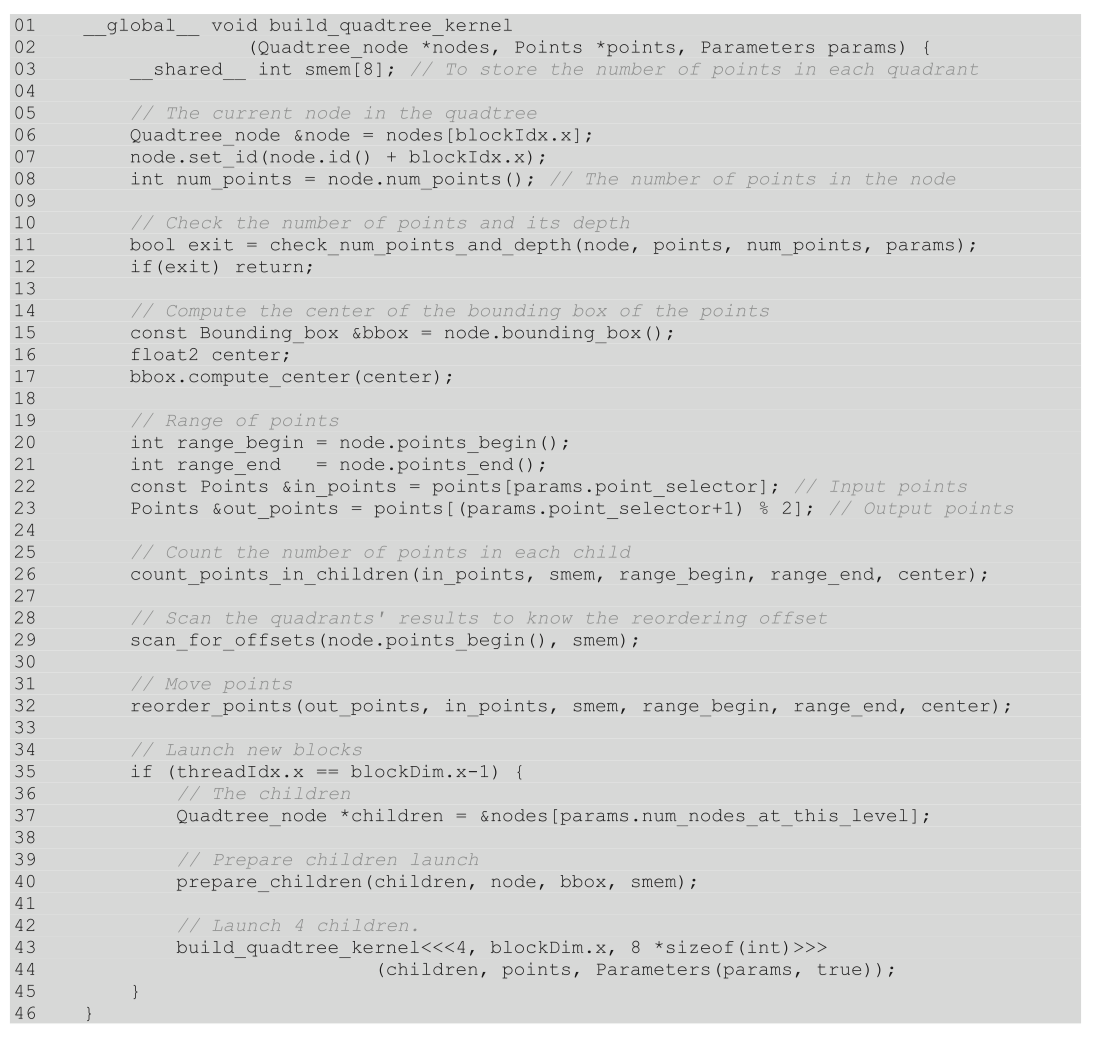
\includegraphics[width=0.9\textwidth]{figs/F21.10.png}
	\caption{\textit{具有动态并行性的四叉树:递归内核(附录A210.1中的支持代码)。}}
\end{figure}

图 21.10 中的内核代码实现了图 21.8 中的流程图。 四叉树是用一个节点数组实现的,
其中每个元素包含四叉树一个节点的所有相关信息(附录 A21.1 中给出的定义)。 
在构建四叉树时,将在内核执行期间创建新节点并将其放入数组中。 内核代码假定节点参数指向节点数组中的下一个可用位置。

\begin{figure}[H]
	\centering
	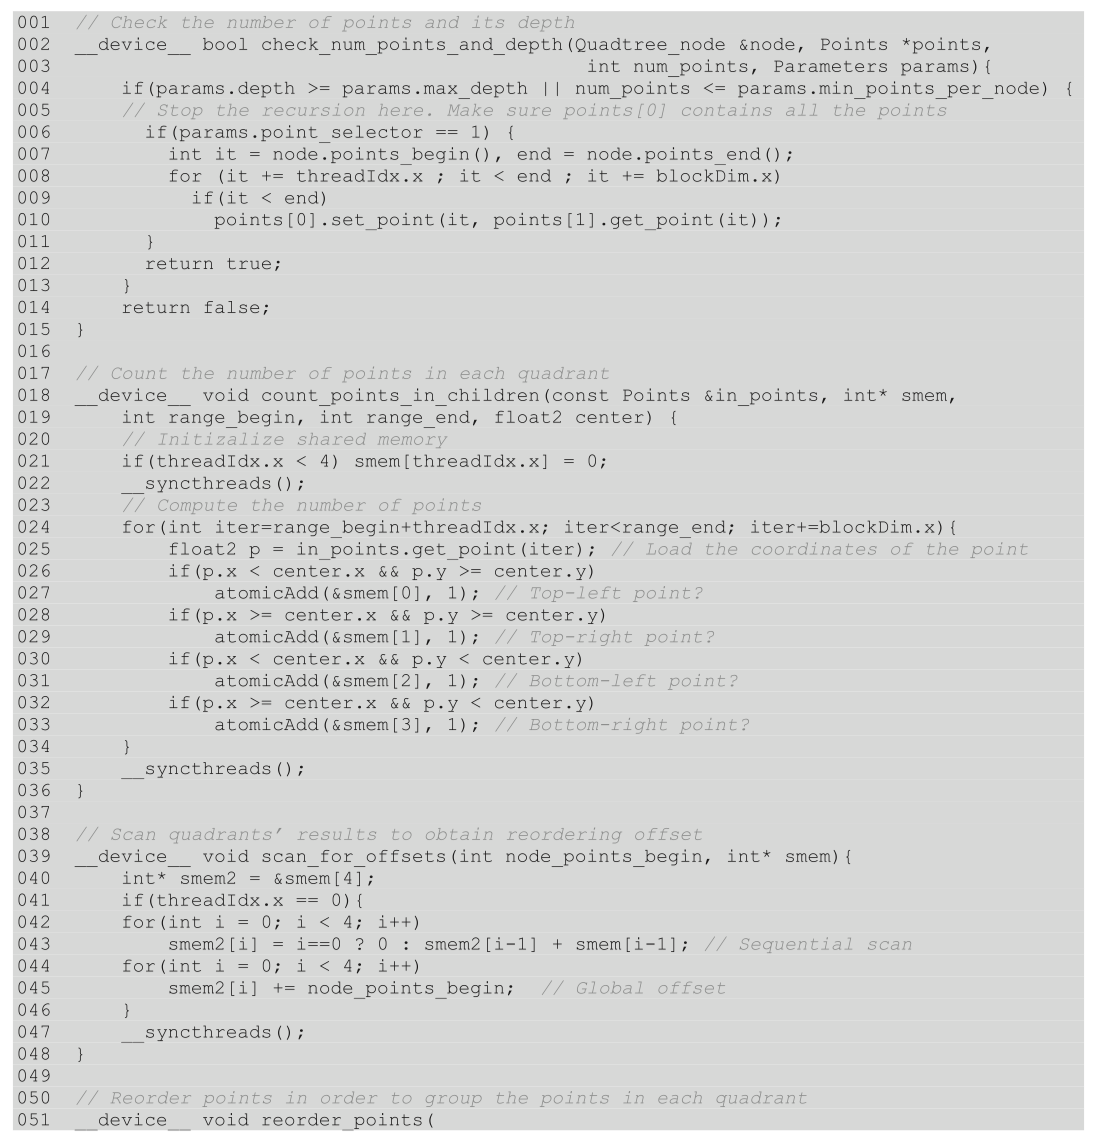
\includegraphics[width=0.9\textwidth]{figs/F21.11-1.png}
	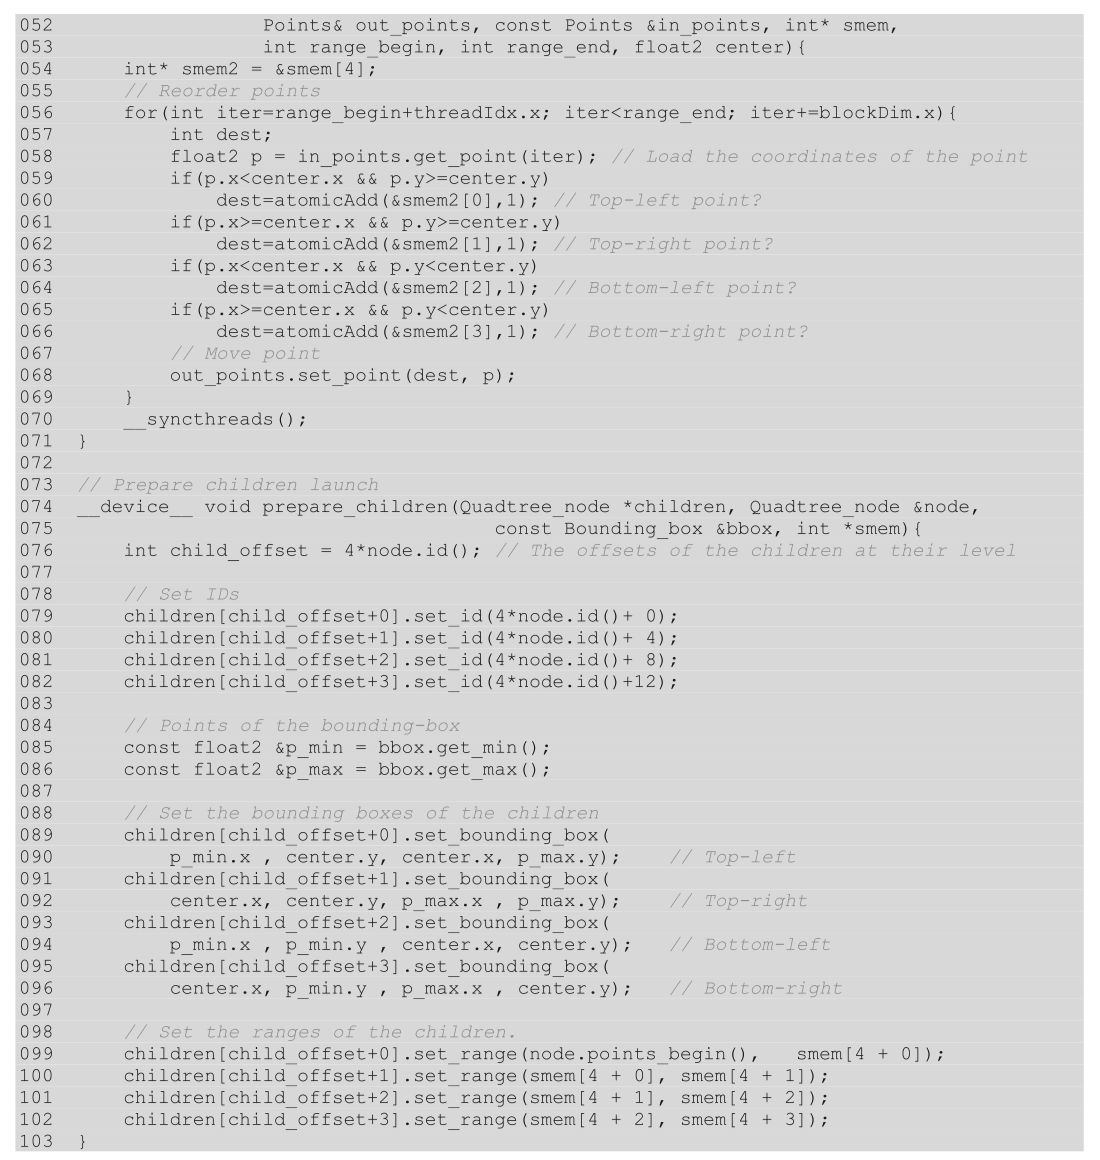
\includegraphics[width=0.9\textwidth]{figs/F21.11-2.png}
	\caption{\textit{具有动态并行性的四叉树:设备函数(附录 A21.1 中的支持代码)。}}
\end{figure}

每个块首先检查其节点(象限)中的点数。 点是一对代表 $x$ 和 $y$ 坐标的浮点(定义见附录 A21.1)。 
如果点数小于或等于最小值或达到最大深度(第 11 行),则块将退出。 
最大深度可以根据应用要求或硬件限制来指定(参见第 12.5 节)。 
在退出之前,如有必要,该块可能需要将其点从缓冲区 1 写入缓冲区 0。 
这是因为四叉树完成后,输出预计位于缓冲区 0 中。 
点从缓冲区 1 到缓冲区 0 的传输是在图 21.11 所示的设备函数 check\_num\_points\_and\_depth( ) 中完成的。

接下来,计算边界框的中心(第 17 行)。 边界框由其左上角和右下角定义。 
当前节点的边界框的左上角和右下角点的坐标由调用者作为节点数据的一部分给出。 中心坐标被计算为这两个角点之间的中点的坐标。 
边界框的定义(包括函数compute\_center())在附录A21.1中给出。 
由于中心将四个象限分开,因此通过与中心点比较,可以确定当前节点中的每个点属于哪个象限。 计算每个象限中的点数(第 26 行)。 
设备函数count\_points\_in\_children()如图21.11所示。 为了清楚起见,这些都被简化了。 
该块的线程协作遍历点范围并使用原子操作来更新每个象限的共享内存中的计数器。

然后调用设备函数 scan\_for\_offsets() (第 29 行)。 如图 21.11 所示,它对共享内存中的四个计数器执行扫描。 
然后,它将父象限的全局偏移量与这些值相加,以得出缓冲区中每个象限组的起始偏移量。

使用象限的偏移量,使用 reorder\_points() 对点重新排序(第 32 行)。 
为简单起见,此设备功能(图 21.11)使用四个象限计数器之一上的原子操作来导出放置每个点的位置。

最后,块的最后一个线程(第 35 行)确定子节点的节点数组中的下一个可用位置(第 37 行),
为子象限准备新节点内容(第 40 行),
并启动一个具有四个子内核的子内核。 线程块(第 43 行)。 
设备函数prepare\_children()通过设置子级边界框的限制和每个象限中的点的范围来为子级准备新的节点内容。 
函数prepare\_children()可以在图13.14(第75行)中找到。

其余定义可在附录 A21.1 中找到。

\subsection{重要考虑因素}
在本节中,我们将简要解释使用动态并行性的程序的执行行为的一些重要注意事项。 
对于程序员来说,为了自信地使用动态并行性,充分理解这些注意事项非常重要。

\subsubsection{内存和数据可见性}
当父线程将内存指针传递给子网格时,它必须确保子网格可以访问所指向的内存,以便子网格不会尝试访问无效内存。 
父线程及其子网格都可以访问的内存包括全局内存、常量内存和纹理内存。 
父线程不应将指向本地内存或共享内存的指针传递给其子网格,因为本地内存和共享内存分别是线程和线程块私有的。

除了确保子网格可以访问父线程传递到子网格的内存之外,程序员还必须知道父线程写入该内存的数据何时对子网格可见,反之亦然 。 
在执行过程中有两个点,父线程和子网格具有相同的内存视图:当父线程启动子网格时,
以及当子网格根据父线程完成同步 API 调用而完成时 线。 换句话说,当父线程启动子网格时,
子网格将看到该启动之前对内存的任何更新,但对于该启动之后的更新则没有这样的保证。 
此外,不能保证子网格对内存所做的任何更新对于父线程都是可见的,直到父线程在子网格完成同步之后。

我们建议读者参阅 CUDA C++ 编程指南,
了解有关父线程和子网格之间的内存和数据可见性的更多详细信息(NVIDIA Corporation,2021)。

\subsubsection{待定启动池配置}
待启动池是一个跟踪正在执行或等待执行的内核的缓冲区。 该池分配了固定数量的空间,
从而支持固定数量的挂起内核调用(默认为 2048)。 如果超过此数字,则会使用虚拟化池,
从而导致显着的速度减慢,速度可能会降低一个数量级或更多。 
为了避免这种减慢,程序员可以通过从主机函数执行 cudaDeviceSetLimit() API 调用来设置 cudaLimitDevRuntimePendingLaunchCount 配置来增加固定池的大小。

例如,在21.3节的贝塞尔曲线计算中,如果N\_LINES设置为4096,那么将启动4096个子网格,因此一半的启动将使用虚拟化池。 
这将导致严重的性能损失。 但是,如果固定大小池设置为4096,则执行时间将大幅减少。

作为一般建议,固定大小池的大小应设置为启动网格的预期数量(如果超过默认大小)。 
在贝塞尔曲线示例中,我们将在调用computeBezierLines\_parent()内核之前调用cudadevicesetLimit (cudaLimitDevRuntimePendingLaunchCount, N\_LINES)。

\subsubsection{Streams}
正如主机代码可以使用流来同时执行内核一样,设备线程可以使用流来启动具有动态并行性的网格。 
流的范围对于创建该流的块来说是私有的。 当内核调用中未指定流时,块中的默认 NULL 流将由所有线程使用。 
这意味着在同一块中启动的所有网格都将被序列化,即使它们是由不同的线程启动的。 
然而,通常情况下,块中不同线程启动的网格是独立的并且可以并发执行。 
因此,如果程序员希望避免序列化造成的性能损失,则必须小心地在每个线程中显式使用不同的流。

第 21.3 节中的贝塞尔曲线示例启动与computeBezierLines\_parent()内核中的父线程一样多的子网格(图21.7中的第19行)。 
如果使用默认的 NULL 流,则由同一父块启动的所有网格都将被序列化。 
因此,与没有动态并行性的原始内核相比,
在启动computeBezierLines\_child()内核时使用默认的NULL流可能会导致并行性急剧减少。

\begin{figure}[H]
	\centering
	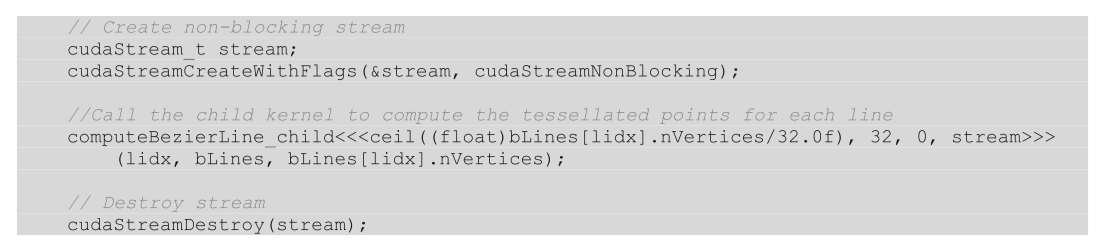
\includegraphics[width=0.9\textwidth]{figs/F21.12.png}
	\caption{\textit{使用命名流启动子内核。}}
\end{figure}

如果需要更多并发性,则必须在每个线程中创建并使用命名流。 图 21.12 显示了应替换图 21.7 中第 19 行的代码。 
使用此代码,从同一线程块启动的内核将被放置在不同的流中并且可以并发运行。 这将更好地利用所有 SM,从而显着减少执行时间。

\subsubsection{嵌套深度}
以动态并行性启动的内核本身可能会调用其他内核,而其他内核又可能会调用其他内核,依此类推。 
我们在 12.4 节的四叉树应用中看到了这样一个内核的例子。 每个下级发射都被视为一个新的嵌套级别,达到的级别总数称为嵌套深度。 
当前硬件支持的最大嵌套深度为24层。 因此,诸如四叉树示例中的内核之类的内核应在决定是否进行动态启动之前检查此限制。

在存在父子同步的情况下,由于系统存储父网格状态所需的内存量,嵌套深度存在额外的限制。 该约束称为同步深度。 
我们建议读者参阅 CUDA C++ 编程指南,了解有关嵌套深度和同步深度的更多详细信息(NVIDIA Corporation,2021)。

\subsection{总结}
CUDA 动态并行性扩展了 CUDA 编程模型,允许内核调用其他内核。 
这允许每个线程动态地发现工作并根据新发现的工作量启动新的网格。 
它还支持线程动态分配设备内存。 
正如我们在贝塞尔曲线计算示例中所示,这些扩展可以实现线程和块之间更好的工作平衡以及更有效的内存使用。 
CUDA 动态并行性还可以帮助程序员实现递归算法,如四叉树示例所示。

除了确保更好的工作平衡之外,动态并行性在可编程性方面还提供了许多优势。 
但是,请务必记住,启动具有少量线程的网格可能会导致 GPU 资源的严重利用不足。 
一般建议是启动具有多个块的子网格,或者如果块的数量很小,则至少启动具有多个线程的块。

类似地,嵌套并行性可以看作是树处理的一种形式,
当树节点很厚(即每个节点部署许多线程)和/或当分支度很大(即每个父节点都有 很多孩子)。 
由于嵌套深度受到硬件的限制,只能有效地实现相对较浅的树。

为了有效地使用动态并行性,程序员需要了解内存内容的可见性、挂起的启动计数和流等细节。 
在动态并行性中仔细使用父级和子级之间的内存和流对于正确执行并在启动子网格时实现预期的并行性水平至关重要。